%HW05.tex
%
% Fifth Homework for Graduate Algebra
% Frank Sottile
%%%%%%%%%%%%%%%%%%%%%%%%%%%%%%%%%%%%%%%%%%%%%%%%%%%%%%%%%%%%%%%%%%%%%%%
\documentclass[12pt]{article}
\usepackage{multicol,amsfonts, amssymb,  mathtools,amsmath}
\usepackage{colordvi,graphicx}
\headheight=8pt
%
\topmargin=-75pt
\textheight=720pt   \textwidth=560pt
\oddsidemargin=-60pt \evensidemargin=-60pt

\pagestyle{empty}

%%%%%%%%%%%%%%%%%%%%%%%%%%%%%%%%%%%%%%%%%%%%
\newcommand{\CC}{{\mathbb C}}
\newcommand{\KK}{{\mathbb K}}
\newcommand{\NN}{{\mathbb N}}
\newcommand{\QQ}{{\mathbb Q}}
\newcommand{\RR}{{\mathbb R}}
\newcommand{\TT}{{\mathbb T}}
\newcommand{\ZZ}{{\mathbb Z}}

\newcommand{\calA}{{\mathcal A}}
\newcommand{\be}{{\bf e}}
\newcommand{\bfi}{{\bf i}}
\newcommand{\bfj}{{\bf j}}

\newcommand{\Hom}{\mbox{Hom}}
\newcommand{\spec}{\mbox{spec}}
\newcommand{\cone}{\mbox{cone}}
\renewcommand{\mod}{{\ \mbox{mod}\ }}

\newcommand{\vect}[2]{(\begin{smallmatrix}#1\\#2\end{smallmatrix})}
\newcommand{\msp}{\hspace{8pt}}
%\newcommand{\Square}{\raisebox{-2pt}{\includegraphics{images/Square.eps}}}
\newcommand{\Square}{\raisebox{-2pt}{\Large$\square$}}

\def\Color#1#2{\special{color push cmyk #1}#2\special{color pop}}
%\def\Indigo#1{\Color{.42 1. 0. .49}{#1}}
\def\Indigo#1{\Color{1. .95 .05 .4}{#1}}
\def\MyViolet#1{\Color{.6 1. 0. .15}{#1}}
\def\TAMU#1{\Color{.15 1. .39 .69}{#1}}

\newcommand{\barsl}{\noindent\begin{minipage}[t]{590pt}
\Indigo{\rule{590pt}{1.2pt}}\vspace{-5.7mm}\\
\MyViolet{\rule{590pt}{1.2pt}}\vspace{-5.7mm}\\
\Blue{\rule{590pt}{1.2pt}}\vspace{-5.7mm}\\
\Green{\rule{590pt}{1.2pt}}\vspace{-5.7mm}\\
\Yellow{\rule{590pt}{1.2pt}}\vspace{-5.7mm}\\
\Orange{\rule{590pt}{1.2pt}}\vspace{-5.7mm}\\
\Red{\rule{590pt}{1.2pt}}\bigskip
\end{minipage}}


\newcommand{\barsn}{\noindent\begin{minipage}[t]{590pt}
\Indigo{\rule{590pt}{1.1pt}}\vspace{-4.5mm}\\
\MyViolet{\rule{590pt}{1.1pt}}\vspace{-4.5mm}\\
\Blue{\rule{590pt}{1.1pt}}\vspace{-4.5mm}\\
\Green{\rule{590pt}{1.1pt}}\vspace{-4.5mm}\\
\Yellow{\rule{590pt}{1.1pt}}\vspace{-4.5mm}\\
\Orange{\rule{590pt}{1.1pt}}\vspace{-4.5mm}\\
\Red{\rule{590pt}{1.1pt}}\bigskip
\end{minipage}}

\def\demph#1{\TAMU{{\sl #1}}}
\def\defcolor#1{\TAMU{#1}}

\begin{document}\LARGE 
\noindent
Algebra \ \ Autumn 2025\vspace{1pt}\\
Frank Sottile\vspace{2pt}\\
\Large 18 September  2025 \hfill
\sf
 Fifth Homework\makebox[20pt][l]{\ }
\normalsize\vspace{10pt}

\noindent
Write your answers neatly, in complete sentences.  
I highly recommend recopying your work before handing it in.
Correct and crisp proofs are greatly appreciated; oftentimes your work can be shortened and made clearer.

\barsn

\noindent\Maroon{{\sf Hand in when you show up for your mid-term exam.}} 

\begin{enumerate}

%%%%%%%%%%%%%%%%%%%%%%%%%%%%%%%%%%%%%%%%%%%%%%%%%%%%%%%%%%%%%%%%%%%%%%%%%%%%%%%%%%%%%%%%%%%%%%%%%%%%
\item   
  Let $m\geq 2$ be an integer.
  Recall that $\defcolor{\ZZ_m}\vcentcolon=\ZZ/m\ZZ=\{0,1,\dotsc,m{-}1\}$.\newline
   Set $\defcolor{\ZZ^*_m}:=\{ k\in \ZZ_m \mid \gcd(k,m)=1\}$.
    These are the cosets of integers that are relatively prime to $m$.
  \begin{enumerate}

   \item  Show that $\ZZ^*_m$ is the set of generators of the cyclic group $\ZZ_m$.
      \vspace{-2pt}

   \item  Show that $\ZZ^*_m$ is a group under multiplication modulo $m$.
         Define $\defcolor{\phi(m)}:=|\ZZ^*_m|$, the order of this group.
          This is Euler's \demph{totient function}, also called Euler's $\phi$-function.\vspace{-2pt}

   \item  Deduce {\bf \defcolor{Euler's Theorem:}}\ 
          If $\gcd(a,m)=1$, then $a^{\phi(m)} \equiv 1\mod m$. \newline
           (That is, $m$ divides $a^{\phi(m)} -1$, equivalently, $a^{\phi(m)}=1$ as elements of $\ZZ_m$.)
            \vspace{-2pt}

   \item  Show that $\phi$ is multiplicative; if $a,b\in\NN$ are relatively prime, ($\gcd(a,b)=1$), then 
           $\phi(ab)=\phi(a)\cdot\phi(b)$.

           Let $p$ be a prime number and show that $\phi(p)=p-1$.
         
          Determine $\phi(p^n)$, where $p$ is a prime and $n>0$ is an integer.

          Deduce a formula for $\phi(m)$ in terms of the factorization of $m$ into a product of powers of distinct
          primes.
          Express this in terms of $m$ and its distinct prime divisors.
      \vspace{-2pt}

   \item   Use (d) to deduce  {\bf \defcolor{Fermat's Little Theorem:}} \newline
           If $p$ is any prime number and $a\in\ZZ$, then $a^p\equiv a\mod p$.

\end{enumerate}
%%%%%%%%%%%%%%%%%%%%%%%%%%%%%%%%%%%%%%%%%%%%%%%%%%%%%%%%%%%%%%%%%%%%%%%%%%%%%%%%%%%%%%%%%%%%%%%%%%%%  

%%%%%%%%%%%%%%%%%%%%%%%%%%%%%%%%%%%%%%%%%%%%%%%%%%%%%%%%%%%%%%%%%%%%%%%%%%%%%%%%%%%%%%%%%%%%%%%%%%%%
\item Let $\defcolor{\mathfrak{H}}\vcentcolon=\{z\in\CC\mid \Im(z)\Red{>} 0\}$ be the upper half plane in the set of complex numbers.
  Let $G\vcentcolon=SL(2,\RR)$, the group of real $2\times 2$ matrices with determinant 1.
  \[
  \mbox{For }z\in\CC\mbox{ and }
  \alpha=\begin{pmatrix}a&b\\c&d\end{pmatrix}\ \in G\ , \mbox{ let } \alpha.z\ \vcentcolon=\frac{az+b}{cz+d}\ .
  \]
  Verify that this defines an action of $G$ on $\mathfrak{H}$, and that the isotropy group of $\sqrt{-1}$ is the group
  \[
  \defcolor{K}\ \vcentcolon=\ \left\{\begin{pmatrix} \cos\theta& \sin\theta \\ -\sin\theta& \cos\theta\end{pmatrix}
  \ \middle| \mbox{ with }\theta\in\RR\right\}\ .
  \]
  of rotation matrices.
  Show that $G$ acts transitively on $\mathfrak{H}$.
%%%%%%%%%%%%%%%%%%%%%%%%%%%%%%%%%%%%%%%%%%%%%%%%%%%%%%%%%%%%%%%%%%%%%%%%%%%%%%%%%%%%%%%%%%%%%%%%%%%%

%%%%%%%%%%%%%%%%%%%%%%%%%%%%%%%%%%%%%%%%%%%%%%%%%%%%%%%%%%%%%%%%%%%%%%%%%%%%%%%%%%%%%%%%%%%%%%%%%%%%
\item   Let $H$ be a subgroup of a group $G$ and define the \demph{core of $H$} to be
\[
    \defcolor{\mbox{core}(H)}\ :=\ \bigcap\{\, {^g}\!H \mid g\in G\}\,,
\]
 the intersection of all conjugates of $H$ by elements of $G$.

 Let $S:=\{xH\mid x\in G\}$ be the set of left cosets of $H$ in $G$.
 For each $g\in G$, define $\defcolor{g_*}\colon S\to S$ by
 $g_*(xH)=gxH$.
 \begin{enumerate}
  \item Show that $g_*$ is an element of the symmetric group on the set $S$, $\mbox{Sym}(S)$.
  \item Show that the map $G\to\mbox{Sym}(S)$ given by $g\mapsto g_*$ is a group homomorphism
         with kernel  $\mbox{core}(H)$. 
 \vspace{-2pt}
 \end{enumerate}
%%%%%%%%%%%%%%%%%%%%%%%%%%%%%%%%%%%%%%%%%%%%%%%%%%%%%%%%%%%%%%%%%%%%%%%%%%%%%%%%%%%%%%%%%%%%%%%%%%%%  


      
\end{enumerate}
%%%%%%%%%%%%%%%%%%%%%%%%%%%%%%%%%%%%%%%%%%%%%%%%%%%%%%%%%%%%%%%%%%%%%%%%%%%%%%%%%%%%%%%%%%%%%%%%%%%%

\end{document}
